\documentclass[aspectratio=169]{beamer}
\usepackage{appendixnumberbeamer}
\usetheme{metropolis}           % Use metropolis theme
\definecolor{fhggreen}{RGB}{23,156,125}
\let\oldemph\textbf
\renewcommand{\textbf}[1]{{\color{mLightBrown}\oldemph{#1}}}

\usepackage{blkarray}
\usepackage{amsmath}
\usepackage{multirow}
\title{
\includegraphics[trim={6cm 7cm 6cm 7cm},clip,width=0.5\textwidth]{reclaim_small}\\\small{Datenspuren 2019}}
\date{21.9.2019}
\author{Martin Schanzenbach}
\institute{\includegraphics[width=.25\textwidth]{aisec_logo.pdf} \hfill \large{GNUnet} 
\includegraphics[trim={0cm 1.5cm 0cm 0cm},clip,width=5em]{gnunet}}
\begin{document}
  \metroset{block=fill,sectionpage=progressbar,numbering=counter}
  \maketitle
 \section{Motivation}

\begin{frame}{Motivation}
  Identity Provider Market:
    \begin{center}
      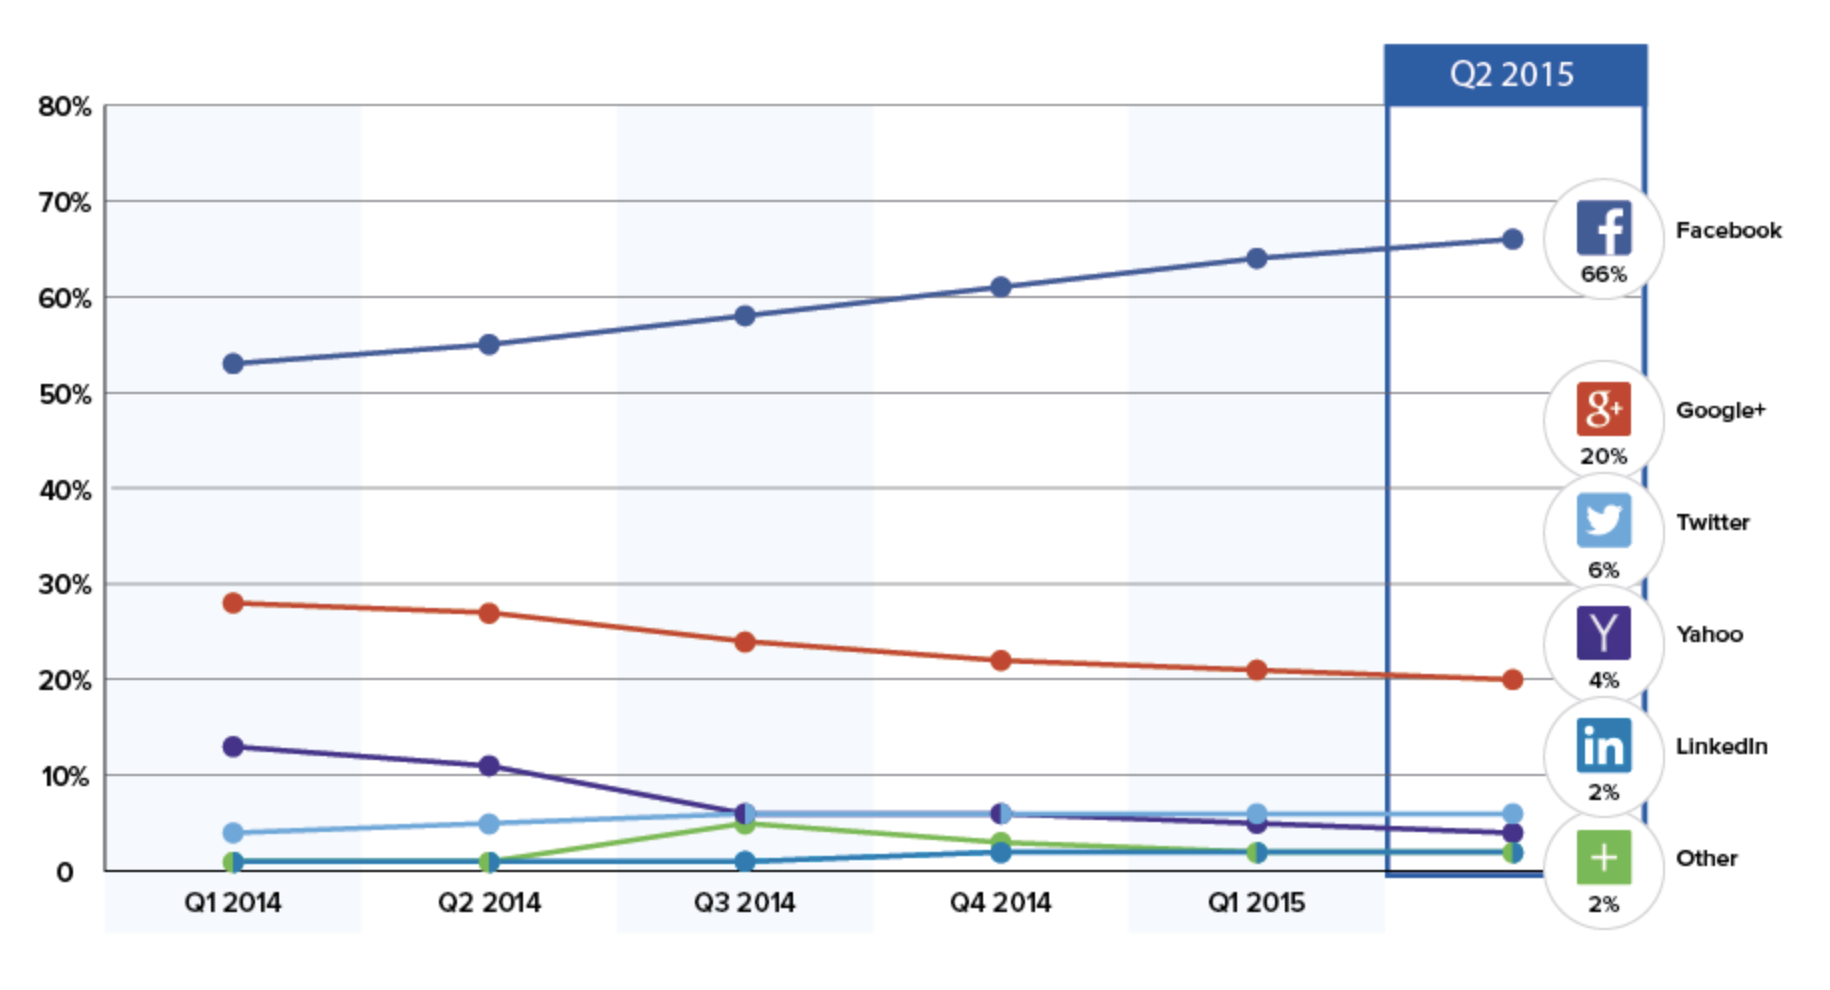
\includegraphics[width=0.9\textwidth]{idp_info}
    \end{center}
    \begin{tiny}
      Source: \url{http://www.gigya.com/blog/the-landscape-of-customer-identity-q2-2015/}
    \end{tiny}
\end{frame}
 \begin{frame}{Motivation}
   Issues:
   \begin{enumerate}
     \item \textbf{Privacy} concerns:
       \begin{itemize}
         \item Targeted advertisement, opinion shaping.
         \item ``Public safety'': Mass surveillance and data collection.
       \end{itemize}
       \pause
     \item \textbf{Liability} risks:
       \begin{itemize}
         \item Data loss through leaks or hacks may result in existential legal implications (GDPR).
       \end{itemize}
       \pause
     \item \textbf{Oligopoly}:
       \begin{itemize}
         \item ``There can be only one (two)''.
         \item IdP market tends to degenerate.
         \item Federation not widely used.
       \end{itemize}
   \end{enumerate}
 \end{frame}

\begin{frame}{Approach}
  \textbf{Primary objective}: We must enable users to exercise their right to digital self-determination:
    \begin{enumerate}
        \pause
      \item Avoid third party services for identity management and data sharing.
        \pause
      \item Open, free and decentralized service which is not under the control of a single organization, consortium or business.
        \pause
      \item Free software.
    \end{enumerate}
    \pause
    $\Rightarrow$ Empower users to \textbf{reclaim} control over their digital identities.
 \end{frame}


 \begin{frame}{What does an IdP do?}
   \begin{enumerate}
     \item Identity provisioning and access control
       \begin{itemize}
         \item Allow management of identities and personal data.
         \item Facilitate sharing of identity data with third parties.
         \item Provide up-to-date information accessible even if user is offline.
         \item Enforce authorization decisions of user.
         \uncover<3->{\item[$\Rightarrow$] \textbf {re:claimID}}
       \end{itemize}
       \pause
       {\color<3->{gray}
     \item Identity information verification and attestation:
       \begin{itemize}
           {\color<3->{gray}
         \item ``this is Alice's email address'': Email provider.
         \item ``this person is living in Germany'': Sovereign state.
         \uncover<3->{\item[$\Rightarrow$] \textbf {Not our department!*}}
           }
       \end{itemize}
       \uncover<3->{\tiny{*We will revisit this further on.}}
       }
   \end{enumerate}
   %\begin{enumerate}
   %  \item Identities and attributes must be shared over a secure, decentralized storage to allow access even of user is offline
   %  \item Access control on data without trusted entity that enforces authorization decisions by user of he is offline
   %\end{enumerate}
 \end{frame}



\section{Introducing 
\includegraphics[trim={6cm 8.2cm 6cm 7cm},clip,width=.4\textwidth]{reclaim_small}}

\begin{frame}
  \begin{itemize}
    \item re:claimID is a \textbf{self-sovereign} personal data sharing system.
    \item Other self-sovereign identity systems you may have head about:
      \begin{itemize}
        \item Sovrin (Hyperledger)\uncover<2->{$\Leftarrow$ \textbf{Permissioned blockchain}}
        \item uPort (Ethereum)\uncover<3->{$\Leftarrow$ \textbf{Data shared off-chain: If user is offline data not accessible}}.
        \item NameID (Namecoin) \uncover<4->{$\Leftarrow$ \textbf{Access control through central server (wat?)}}

      \end{itemize}
    \uncover<5->{\item[!] re:claimID does \textbf{not} require a blockchain, is fully decentralized and allows asynchronuous data access.}
  \end{itemize}
\end{frame}



\begin{frame}{In a nutshell}
  \begin{minipage}[m]{0.40\textwidth}
    \centering
    \centering
    
\includegraphics[trim={6cm 7cm 6cm 7cm},clip,width=1\textwidth]{reclaim_small}
  \end{minipage}
  \begin{minipage}[m]{0.2\textwidth}
    \centering
    \Huge {\color{black} =}
  \end{minipage}
  \begin{minipage}[m]{0.25\textwidth}
    \centering
    {\large \textbf{Decentralized directory service}}\\
    \vspace{1em}
    {\Huge \color{black} +}\\
    \vspace{1em}
    {\large \textbf{Cryptographic access control}}
  \end{minipage}
\end{frame}

\begin{frame}{Directory services?}
  \begin{center}
    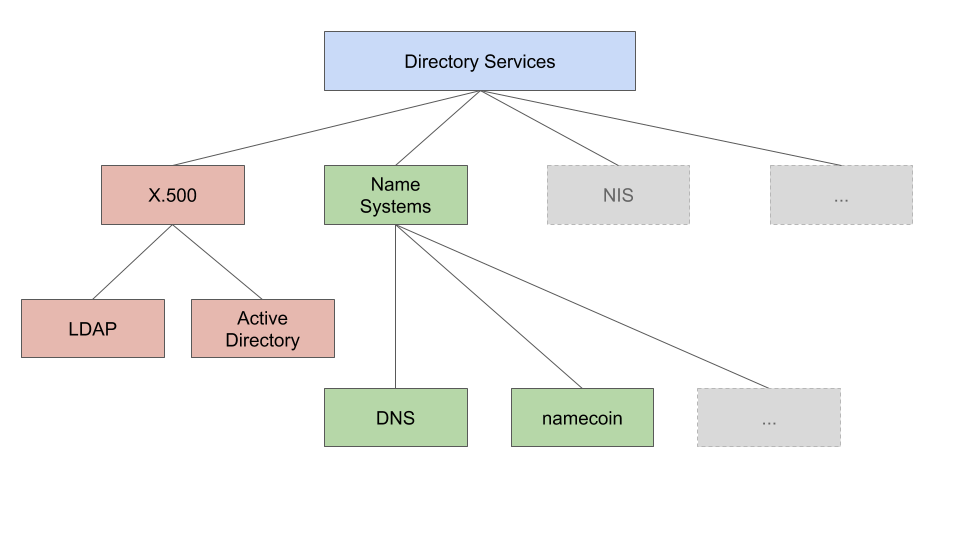
\includegraphics[width=1\textwidth]{directories}
  \end{center}
\end{frame}


\begin{frame}{In a nutshell}
  \begin{itemize}
    \item Decentralized directory service
      \begin{itemize}
        \item Secure \textbf{name system} with open name registration.
        \item Idea ``borrowed'' from NameID.
        \item Example: nslookup email.bob.org $\Rightarrow$ ``bob@example.com''
        \item Our implementation uses the \textbf{GNU Name System (GNS)}
      \end{itemize}
      \pause
    \item Cryptographic access control layer
      \begin{itemize}
        \item Provided by GNS through encrypted and signed resource records.
        \item Protects identity data from unwanted disclosure and allows users to enforce access control.
      \end{itemize}
  \end{itemize}
  %\begin{enumerate}
  %  \item Identities and attributes must be shared over a secure, decentralized storage to allow access even of user is offline
  %  \item Access control on data without trusted entity that enforces authorization decisions by user of he is offline
  %\end{enumerate}
\end{frame}

%\begin{frame}{Centralized Storage, centralized IdP}
%  \includegraphics[width=1\textwidth]{idp_traditional}
%\end{frame}
%\begin{frame}{Decentralized Storage, centralized IdP}
%  \includegraphics[width=1\textwidth]{idp_nameid}
%\end{frame}
%\begin{frame}{reclaimID}
%  \includegraphics[width=1\textwidth]{idp_gnuid}
%\end{frame}
%


\section{How does it work}

\begin{frame}{Managing and publishing identity information}
  \centering
  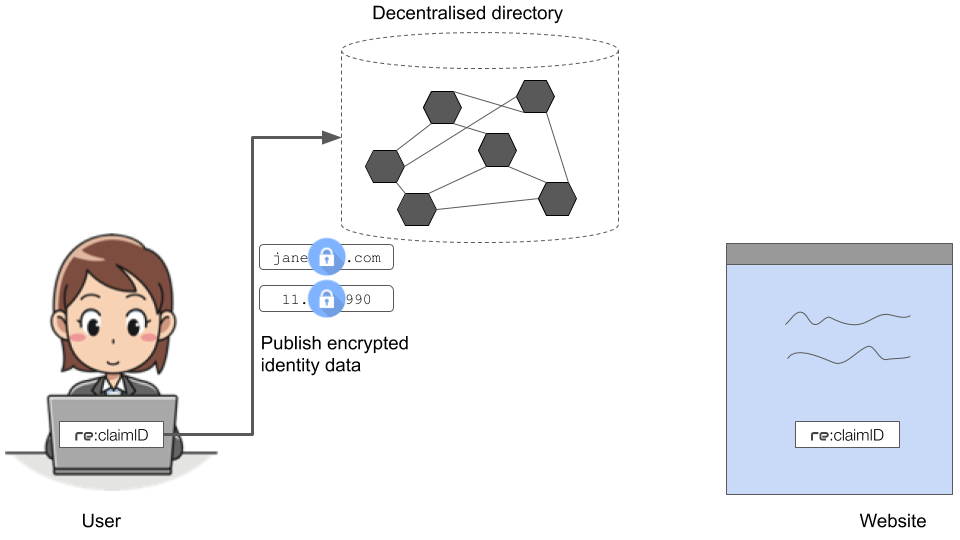
\includegraphics[width=1\textwidth]{Reclaim-2}
\end{frame}

\begin{frame}{The GNU Name System}
  \begin{itemize}
    \item In GNS, a namespace is defined by a public/private EC key pair:
      \begin{itemize}
        \item $x$: Private key
        \item $P$: Public key
        \item $G$: Generator of the curve
        \item $n$: Group order
      \end{itemize}
      \pause
    \item Records are encrypted and signed using keys derived from $(x,P)$.
      \pause
    \item Encrypted records are published in a distributed hash table (under key $q$).
      \pause
    \item Any peer is able to verify the signature as the corresponding derived public key is also published.
    \pause
    \item Records can only be resolved and decrypted if the true identity and the label is known.
    \pause
    \item[$\Rightarrow$] Namespaces \textbf{cannot} be enumerated and queries/responses \textbf{cannot}* be observed.
  \end{itemize}
  \tiny{*Unless label and identity are known.}
\end{frame}

\begin{frame}{Identity attributes in GNS}
  Users may create a namespace  $(x,P)$ and use it as a digital identity containing personal information:
  \begin{table}[h]
    \begin{tabular}{|c|c|c|}
      \hline
      Label & Record Type & Value \\\hline\hline
      $l_{email}$    & \texttt{ATTR} & ``email=alice@example.com''\\\hline
      $l_{name}$    & \texttt{ATTR} & ``name=Alice Doe''\\\hline
      $l_{dob}$  & \texttt{ATTR}    & ``dob=1.3.1987'' \\\hline
    \end{tabular}
  \end{table}
  where the labels are \textbf{random secret values} with high entropy.
\end{frame}


\begin{frame}{Publishing information}
  Given a namespace $(x,P)$, we can treat labels as shared secrets in order to selectively disclose information.

  %\setlength{\jot}{4.5pt}
  \[
    \def\arraystretch{1.1}
    \begin{blockarray}{r@{\;}l}
      \begin{block}{r@{\;}l}
        h &:= Hash(l_{attr},P) \\[\jot]
      \end{block}
      \pause
      \\
      \begin{block}{\Left{\textbf{DHT key }}{\{}r@{\;}l}
        q &:= H(hP) \\
      \end{block}
      \pause
      \\
      \begin{block}{\Left{\textbf{Encryption }}{\{}r@{\;}l}
        k &:= HKDF(l_{attr},P) \\[\jot]
        Record &:= Enc_k(Data) \\[\jot]
      \end{block}
      \pause
      \\
      \begin{block}{\Left{\textbf{Signature }}{\{}r@{\;}l}
        d &:= h\cdot x~mod~n \\[\jot]
        Signature &= Sig_d(Record) \\[\jot]
      \end{block}
    \end{blockarray}
  \]
\end{frame}

\begin{frame}{Authorizing access}
  \centering
  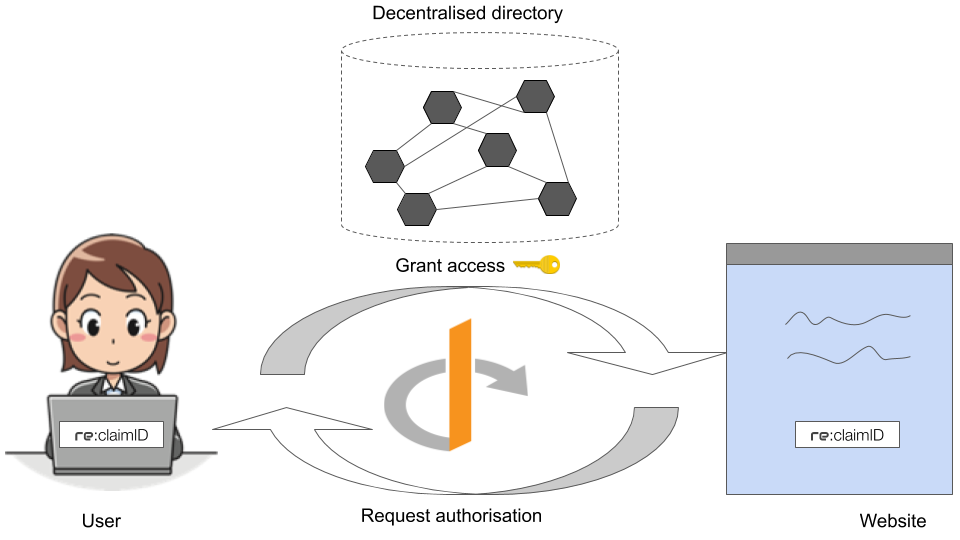
\includegraphics[width=1\textwidth]{Reclaim-3}
\end{frame}


\begin{frame}{Authorizing access}
  \begin{table}[h]
    \begin{tabular}{|c|c|c|}
      \hline
      Label & Record Type & Value \\\hline\hline
      $l_{email}$    & \texttt{ATTR} & ``email=alice@doe.com''\\\hline
      $l_{name}$    & \texttt{ATTR} & ``name=Alice Doe''\\\hline
      $l_{dob}$  & \texttt{ATTR}    & ``dob=1.3.1987'' \\\hline\pause
      \multirow{2}{*}{\textbf{$l_{ticket}$}}    & \texttt{ATTR\_REF} & $l_{email}$\\\cline{2-3}
      & \texttt{ATTR\_REF} & $l_{dob}$\\\hline
    \end{tabular}
  \end{table}
  \begin{itemize}
    \item For each authorized party, the user publishes reference records under the secret label \textbf{$l_{ticket}$}
    \item \textbf{$l_{ticket}$} can be shared with a third party in order to authorize access to email and dob.
    \item Indirection enables us to revoke tickets.
  \end{itemize}
\end{frame}


%\begin{frame}{Transfer keys}
%  \centering
%  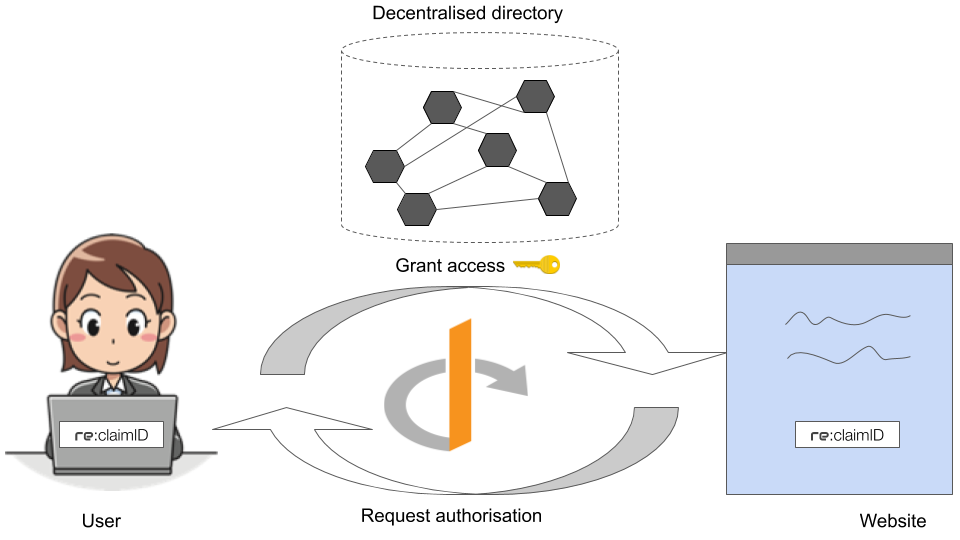
\includegraphics[width=1\textwidth]{Reclaim-3}
%\end{frame}


\begin{frame}{Retrieve and decrypt attributes}
  \centering
  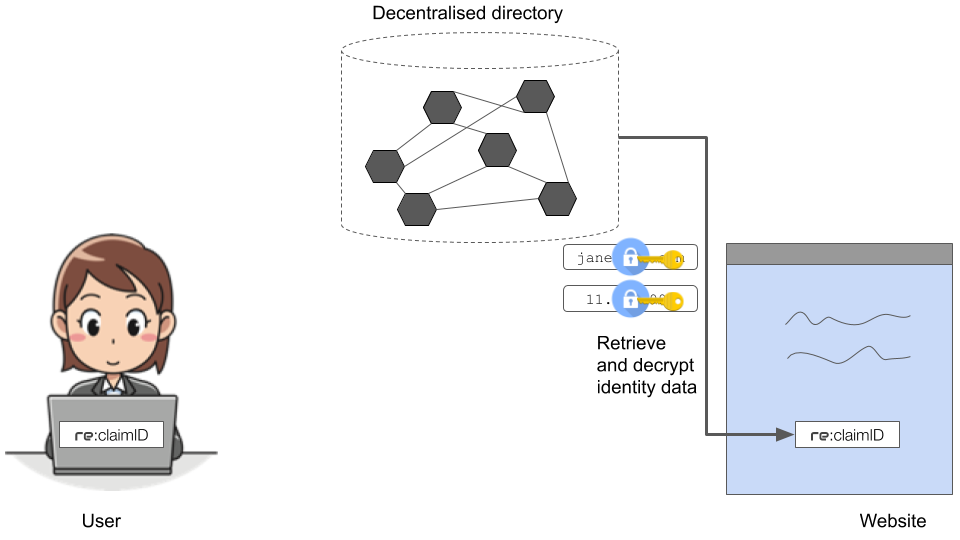
\includegraphics[width=1\textwidth]{Reclaim-4}
\end{frame}

\begin{frame}{Retrieving information}
  Given an identity with public key $P$, we can retrieve references using \textbf{$l_{ticket}$} and subsequently identity info from GNS.

  %\setlength{\jot}{4.5pt}
  \[
    \def\arraystretch{1.1}
    \begin{blockarray}{r@{\;}l}
      \begin{block}{r@{\;}l}
        h &:= Hash(l_{ticket},P) \\[\jot]
      \end{block}
      \pause
      \\
      \begin{block}{\Left{\textbf{DHT key }}{\{}r@{\;}l}
        q &:= H(hP) \\[\jot]
      \end{block}
      \pause
      \\
      \begin{block}{\Left{\textbf{Record decryption }}{\{}r@{\;}l}
        k &:= HKDF(l_{ticket},P) \\[\jot]
        Data &:= Dec_k(Record) \\[\jot]
      \end{block}
    \end{blockarray}
  \]
\end{frame}

\begin{frame}{Integration}
  \begin{itemize}
    \item re:claimID implements the OpenID Connect protocol.
    \item For websites, it is just like integrating any other IdP (e.g. Google)
    \item For users, the authorization flow looks just like with anny other OpenID Connect IdP.
  \end{itemize}
\end{frame}

\begin{frame}{}
  \centering
  Demo
\end{frame}


\section{Who sais that, anyway?}

\begin{frame}{Attestations}
  \centering
  \begin{itemize}
    \item Sometimes we need third party assurances to establish trust in identities.
      \pause
    \item Currently, IdPs such as Facebook/Google implicitly provide this assurance (i.e. vouch for the truthfulness and correctness).
      \pause
    \item Claim: Those parties are not actually the authorities over (most of) your personal data! Examples:
      \begin{itemize}
        \item Real name (State/Self-asserted/Other organization)
        \item Phone number (Provider)
        \item Address (State/Self-asserted)
        \item Citizenship (State)
        \item Age (State)
        \item Email address (Mail provider)
      \end{itemize}
  \end{itemize}
\end{frame}

\begin{frame}{Attestations}
  \centering
  \begin{itemize}
    \item What users actually need is a \textbf{collection of credentials}.
      \pause
    \item Those credentials are issued by a \textbf{variety of different entities}, including the user.
      \pause
    \item Credentials are ideally \textbf{preserving the privacy} of the individual, e.g. using zero-knowledge proofs.
      \pause
    \item Those ideas are already finding their way into standards:
      \begin{itemize}
        \item W3C: ``Verifiable Credentials''
        \item OpenID Connect: ``Aggregated Claims'' \uncover<5->{$\Leftarrow$ \textbf{working on it}.}
      \end{itemize}
  \end{itemize}
\end{frame}


%\begin{frame}{Authorization protocol and key transfer}
%  \centering
%  \begin{center}
%    \begin{minipage}[m]{0.8\textwidth}
%      \centering
%      
\includegraphics[trim={6cm 6.5cm 6cm 7cm},clip,width=0.5\textwidth]{reclaim_small}
%      \vspace{0.5cm}
%    \end{minipage}
%
%    \begin{minipage}[m]{0.8\textwidth}
%      \centering
%      %{\Huge \color{fhggreen} $\heartsuit$}
%      
\includegraphics[clip,width=1.5cm]{handshake}
%    \end{minipage}
%
%    \begin{minipage}[m]{0.7\textwidth}
%      \centering
%      \vspace{0.5cm}
%      %\includegraphics[width=0.2\textwidth]{openid_logo}
%      \huge{OpenID Connect}
%    \end{minipage}
%  \end{center}
%\end{frame}

\section{Using re:claimID}
\begin{frame}{Installing re:claimID}
  \begin{enumerate}
    \item Install the webextension: \url{https://addons.mozilla.org/firefox/addon/reclaimid/}
    \item \uncover<2->{Install \textbf{GNUnet} $>=0.11.6$}
  \end{enumerate}
  \pause
  \uncover<1-2>{
    \begin{center}
      
\includegraphics[height=0.4\textwidth]{iu.jpg}
    \end{center}
  }
\end{frame}

\begin{frame}{Installing re:claimID}
  Get help installing GNUnet and/or re:claimID at our workshop today!
  \begin{itemize}
    \item Right after this.
    \item Time: 12:15 PM -- 15:00 PM
    \item Location: Seminarraum
  \end{itemize}
\end{frame}


\section{Summary}

\begin{frame}{Status}
  \begin{itemize}
    \item Get it at \url{https://reclaim-identity.io}.
    \item Demo websites exist:
      \begin{itemize}
        \item \url{https://demo.reclaim-identity.io}
        \item \url{https://eusec.clouditor.io}
      \end{itemize}
    \item Roadmap:
      \begin{itemize}
        \item User-friendly packaging (of GNUnet)
        \item Ship GNUnet inside browser plugin (yes, that might even work).
        \item ``1.0'' by end of 2019
      \end{itemize}
  \end{itemize}
  \begin{center}
      \end{center}
\end{frame}


\begin{frame}
  \begin{center}
    Questions?\\
    \vspace{2cm}
    \url{https://reclaim-identity.io}\\
    \url{https://gnunet.org}\\
    \vspace{1em}
    {\tiny
    \texttt{schanzen@aisec.fraunhofer.de}\\
    \texttt{6665~201E~A925~7CC6~8FDE~77E8~8433~5131~EA3D~ABF0}\\
    -- or --\\
    \texttt{schanzen@gnunet.org}\\
    \texttt{3D11~063C~10F9~8D14~BD24~D147~0B09~98EF~86F5~9B6A}\\
    }
  \end{center}
\end{frame}

\appendix

\begin{frame}{References}
  \centering
  {\small
  \begin{enumerate}
    \item {Matthias Wachs, Martin Schanzenbach and Christian Grothoff. {\em A Censorship-Resistant, Privacy-Enhancing and Fully Decentralized Name System}. {\bf 13th Intern
      ational Conference on Cryptology and Network Security}, 2014.}
    \item {Martin Schanzenbach, Georg Bramm, Julian Schütte. {\em reclaimID: Secure, Self-Sovereign Identities Using Name Systems and Attribute-Based Encryption}. {\bf 17th
      IEEE International Conference On Trust, Security And Privacy In Computing And Communications (TrustCom)}, 2018}
  \end{enumerate}
  }
\end{frame}



%\begin{frame}{NameID}
%  NameID:
%  \begin{center}
%    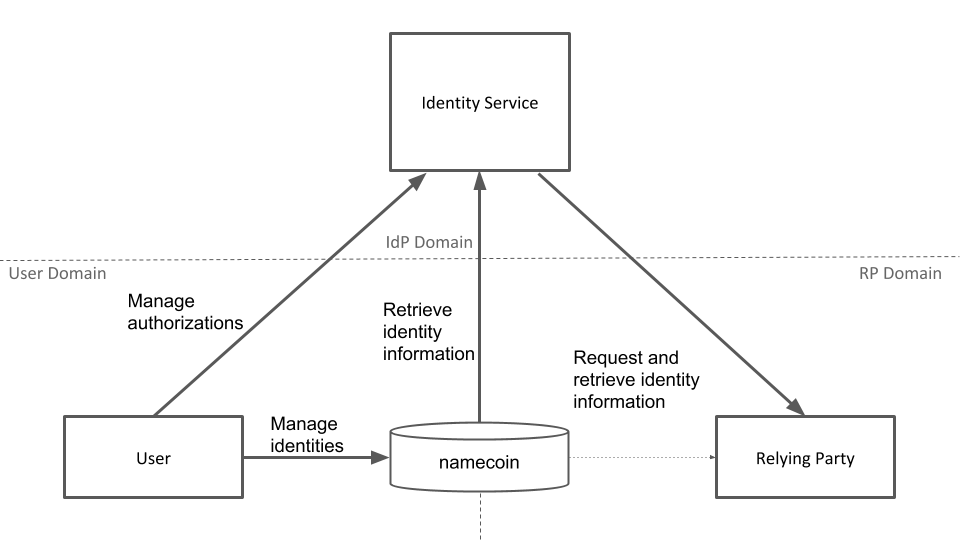
\includegraphics[width=1\textwidth]{nameid}
%  \end{center}
%\end{frame}
%
%\begin{frame}{Performance}
%  Impact of name system caches on successive attribute resolution.
%  \begin{center}
%    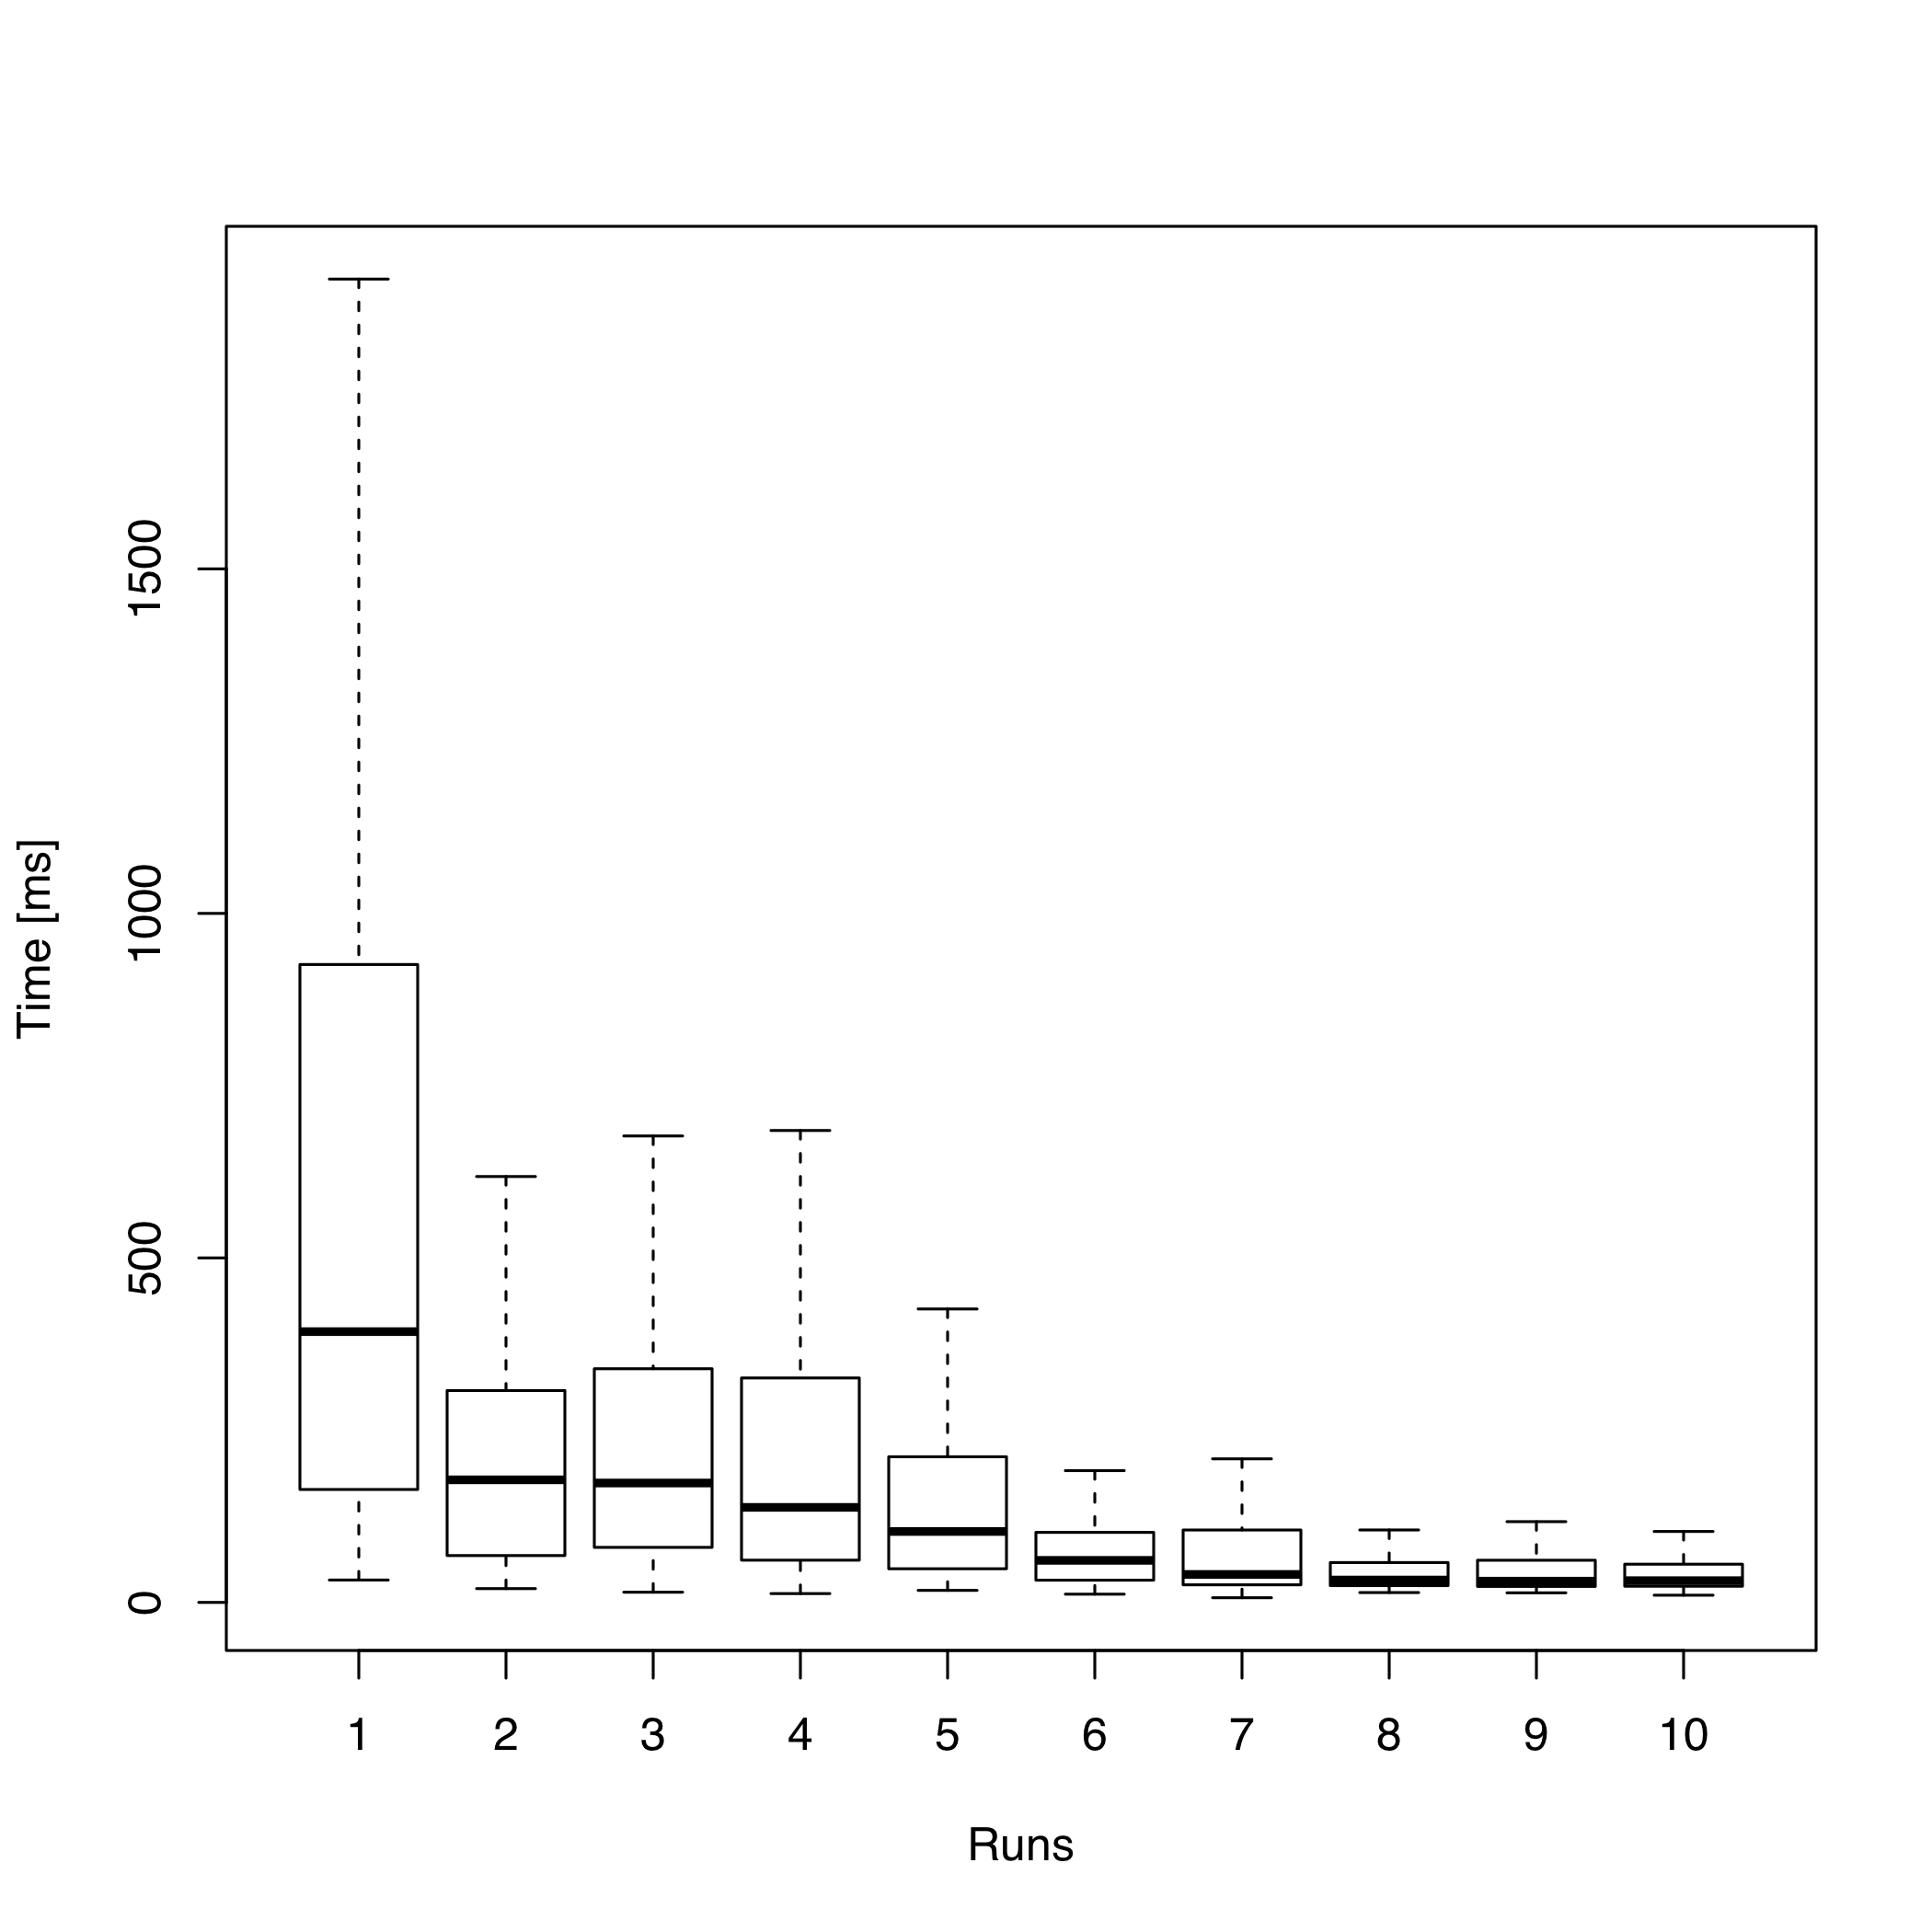
\includegraphics[width=0.7\textwidth]{attr_perf_plot_100}
%  \end{center}
%
%\end{frame}
%
%\begin{frame}{Performance}
%  Attribute resolution performance depending on network size.
%  \begin{center}
%    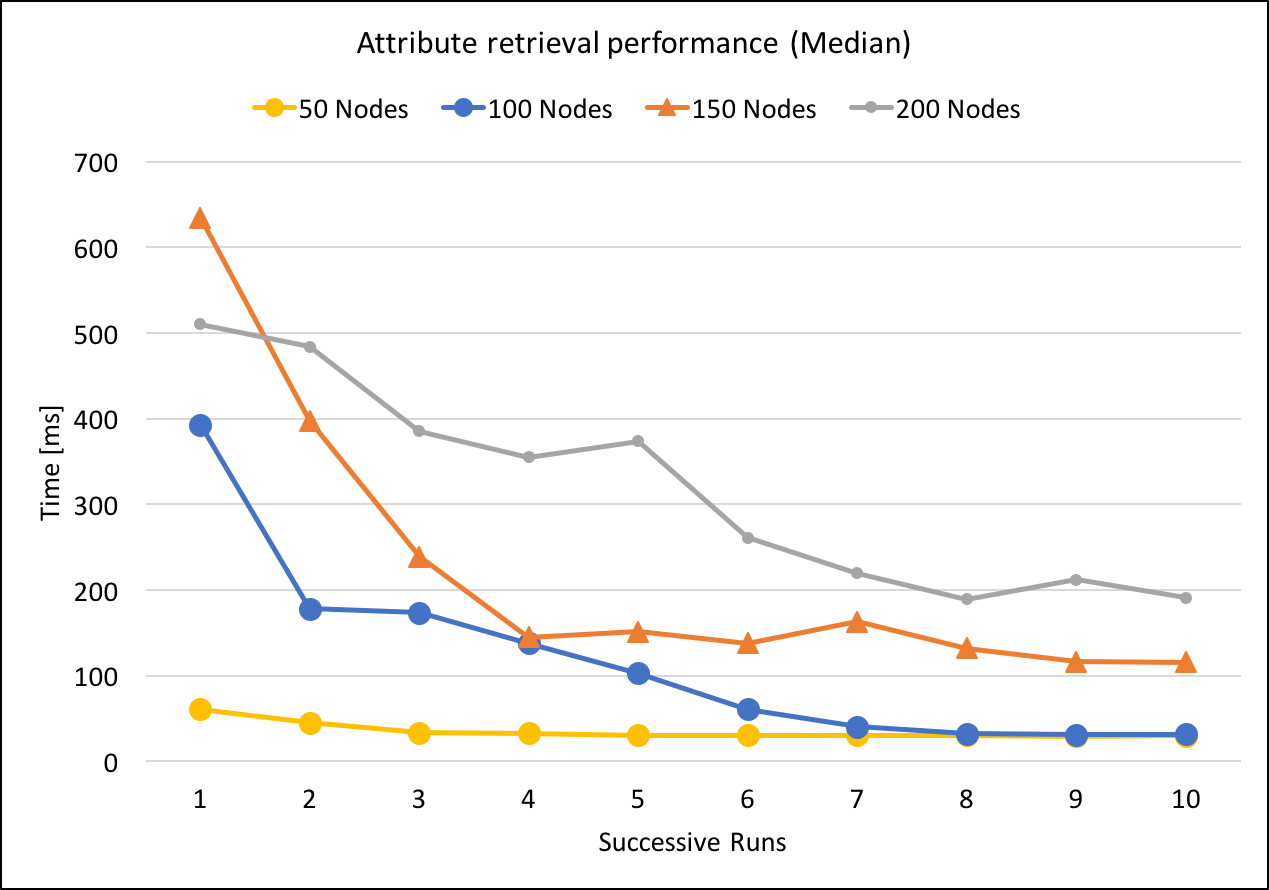
\includegraphics[width=0.8\textwidth]{perf_attrs.png}
%  \end{center}
%
%\end{frame}
%

\end{document}
